% !TeX spellcheck = es_ES
% !TeX encoding = UTF-8
\documentclass[10pt, a4paper]{article}

% ----- packages -----
\usepackage{amsmath} % AMS mathematical facilities for LaTeX
\usepackage{enumitem} % Control layout of itemize, enumerate, description
\usepackage{fancyhdr} % Extensive control of page headers and footers in LaTeX2
\usepackage{geometry} % Flexible and complete interface to document dimensions
\usepackage{graphicx} % Enhanced support for graphics
\usepackage{hyperref} % Extensive support for hypertext in LaTeX
\usepackage{parskip} % Layout with zero \parindent, non-zero \parskip
\usepackage{titlesec} % Select alternative section titles
\usepackage{multirow} % Create tabular cells spanning multiple rows

% ----- pdf metadata -----
\hypersetup{
	pdftitle={Hoja de Referencia Matemáticas Financieras},
	pdfsubject={Financial Mathematics Cheat Sheet - marcelomijas - CC-BY-4.0},
	pdfauthor={Marcelo Moreno Porras},
	pdfkeywords={latex, economics, cheatsheet, financial-mathematics}
}

% ----- custom commands -----
% simple interest formulas
\newcommand{\Sif}{$C_{n} = C_{0} \cdot (1 + i \cdot n)$}
\newcommand{\SifRateim}{$i_{m} = \dfrac{i}{m}$}
\newcommand{\SifSolveCo}{$C_{0} = \dfrac{C_{n}}{1 + i \cdot n}$}
\newcommand{\SifSolvei}{$i = \dfrac{\frac{C_{n}}{C_{0}} - 1}{n}$}
\newcommand{\SifSolven}{$n = \dfrac{\frac{C_{n}}{C_{0}} - 1}{i}$}
% compound interest formulas
\newcommand{\Cif}{$C_{n} = C_{0} \cdot (1 + i)^{n}$}
\newcommand{\CifRateim}{$i_{m} = (1 + i)^{1 / m} - 1$}
\newcommand{\CifRatei}{$i = (i_{m} + 1)^{m} - 1$}
\newcommand{\CifSolveCo}{$C_{0} = \dfrac{C_{n}}{(1 + i)^{n}}$}
\newcommand{\CifSolvei}{$i = \left(\dfrac{C_{n}}{C_{0}}\right)^{1 / n} - 1$}
\newcommand{\CifSolven}{$n = \dfrac{\log{\left(\frac{C_{n}}{C_{0}}\right)}}{\log{(1 + i)}}$}
% simple discount formulas
\newcommand{\Sdf}{$C_{0} = C_{n} (1 - d \cdot n)$}
\newcommand{\SdfRatedm}{$d_{m} = \dfrac{d}{m}$}
\newcommand{\Sdfr}{\textbf{Racional} \quad $C_0 = \dfrac{C_{n}}{1 + i \cdot n}$}
% compound discount formula
\newcommand{\Cdf}{$C_{0} = C_{n} \cdot (1 - d)^{n}$}
% temporal unitary rent formulas
\newcommand{\TurfPoa}{$a_{n \rceil i} = \dfrac{1 - (1 + i)^{-n}}{i}$}
\newcommand{\TurfPos}{$S_{n \rceil i} = a_{n \rceil i} \cdot (1 + i)^{n}$}
\newcommand{\TurfPra}{$\ddot{a}_{n \rceil i} = (1 + i) \cdot a_{n \rceil i}$}
\newcommand{\TurfPrs}{$\ddot{S}_{n \rceil i} = (1 + i) \cdot S_{n \rceil i}$}
% perpetual unitary rent formulas
\newcommand{\PurfPoa}{$a_{\infty \rceil i} = \dfrac{1}{i}$}
\newcommand{\PurfPra}{$\ddot{a}_{\infty \rceil i} = (1 + i) \cdot a_{\infty \rceil i}$}
% temporal geometric rent formulas
\newcommand{\TgrfPoA}{$A(C;q)_{n \rceil i} =
	\begin{cases}
		C \cdot \dfrac{1 - \left( \dfrac{q}{1 + i} \right)^n}{1 + i - q} & \mathrm{si} \quad q \neq 1 + i \\
		C \cdot \dfrac{n}{1 + i}                                         & \mathrm{si} \quad q = 1 + i
	\end{cases}$}
\newcommand{\TgrfPoS}{$S(C;q)_{n \rceil i} = A(C;q)_{n \rceil i} \cdot (1 + i)^n$}
\newcommand{\TgrfPrA}{$\ddot{A}(C;q)_{n \rceil i} = (1 + i) \cdot A(C;q)_{n \rceil i}$}
\newcommand{\TgrfPrS}{$\ddot{S}(C;q)_{n \rceil i} = (1 + i) \cdot S(C;q)_{n \rceil i}$}
% perpetual geometric rent formulas
\newcommand{\PgrfPoA}{$A(C;q)_{\infty \rceil i} =
	\begin{cases}
		C \cdot \dfrac{1}{1 + i - q} & \mathrm{si} \quad q < 1 + i    \\
		\mathrm{Infinito}            & \mathrm{si} \quad q \geq 1 + i
	\end{cases}$}
\newcommand{\PgrfPrA}{$\ddot{A}(C;q)_{\infty \rceil i} = (1 + i) \cdot A(C;q)_{\infty \rceil i}$}
% constant
\newcommand{\Const}{Constante}
% loan french type
\newcommand{\Lfta}{$a = \dfrac{C_{0}}{a_{n \rceil i}}$}
\newcommand{\LftA}{$A_{s} = A_{1} \cdot (1 + i)^{s - 1}$}
\newcommand{\LftC}{$C_{0} = A_{1} \cdot S_{n \rceil i}$}
\newcommand{\LftCRec}{$C_{s} = C_{s - 1} \cdot (1 + i) - a$}
\newcommand{\LftCPro}{$C_{s} = a \cdot a_{n - s \rceil i}$}
\newcommand{\LftCRet}{$C_{s} = C_{0} \cdot (1 + i)^{s} - a \cdot S_{s \rceil i}$}
% loan american type
\newcommand{\Latas}{$a_{s} = I_{s} = C_{0} \cdot i_{s} \quad \mathrm{si} \quad s \neq n$}
\newcommand{\Latan}{$a_{n} = I_{n} + C_{0} = C_{0} \cdot i_{s} + C_{0} \quad \mathrm{si} \quad s = n$}
\newcommand{\LatAs}{$A_{s} = 0 \quad \mathrm{si} \quad s \neq n$}
\newcommand{\LatAn}{$A_{n} = C_{0} \quad \mathrm{si} \quad s = n$}
\newcommand{\LatCs}{$C_{s} = C_{0} \quad \mathrm{si} \quad s \neq n$}
\newcommand{\LatCn}{$C_{n} = 0 \quad \mathrm{si} \quad s = n$}
% loan italian type
\newcommand{\Lita}{$a_{s + 1} = a_{s} - i \cdot A$}
\newcommand{\LitI}{$I_{s + 1} = I_{s} - i \cdot A$}
\newcommand{\LitA}{$A = \dfrac{C_{0}}{n}$}
\newcommand{\LitCRec}{$C_{s} = C_{s - 1} - A$}
\newcommand{\LitCPro}{$C_{s} = C_{n - s} \cdot A$}
\newcommand{\LitCRet}{$C_{s} = C_{0} - s \cdot A$}
% loan geometrical type
\newcommand{\Lgta}{$a = \dfrac{C_{0}}{A(1;q)_{n \rceil i}}$}
\newcommand{\LgtCRec}{$C_{s} = C_{s - 1} \cdot (1 + i) - a \cdot q^{s - 1}$}
\newcommand{\LgtCPro}{$C_{s} = A(a \cdot q^{s};q)_{n - s \rceil i}$}
\newcommand{\LgtCRet}{$C_{s} = C_{0} \cdot (1 + i)^{s} - S(a;q)_{s \rceil i}$}
% vertical text
\newcommand{\vtext}[1]{
	\rotatebox[origin=c]{90}{#1}
}

% ----- page customization -----
\geometry{margin=1cm} % margins config
\pagenumbering{gobble} % remove page numeration
\setlength{\parskip}{0cm} % paragraph spacing
% title spacing
\titlespacing{\section}{0pt}{2ex}{1ex}

% ----- footer -----
\pagestyle{fancy}
\renewcommand{\headrulewidth}{0pt}
\cfoot{\href{https://github.com/marcelomijas/financial-math-cheatsheet}{\normalfont \footnotesize FM-25.01-ES - github.com/marcelomijas/financial-math-cheatsheet - CC-BY-4.0 license}}
\setlength{\footskip}{12pt}

% ----- document -----
\begin{document}

\begin{center}
	\textbf{\LARGE \href{https://github.com/marcelomijas/financial-math-cheatsheet}{Hoja de Referencia Matemáticas Financieras}}

	{\footnotesize Por Marcelo Moreno Porras - Universidad Rey Juan Carlos}
\end{center}

\section*{Capitalización y descuento}

\begin{center}
	\renewcommand{\arraystretch}{2.5}
	\begin{tabular}{|c|cc|cc|}
		\hline
		                                            &    \multicolumn{2}{c|}{\textbf{Capitalización}}     &       \multicolumn{2}{c|}{\textbf{Descuento}}       \\ \hline
		 \multirow{2}{*}{\vtext{\textbf{Simple}}}   & \multirow{2}{*}{\Sif} & \multirow{2}{*}{\SifRateim} & \Sdf &                  \SdfRatedm                  \\
		                                            &                       &                             &         \multicolumn{2}{c|}{\textbf{\Sdfr}}         \\ \hline
		\multirow{2}{*}{\vtext{\textbf{Compuesta}}} & \multirow{2}{*}{\Cif} &         \CifRateim          & \multicolumn{2}{c|}{\multirow{2}{*}{\textbf{\Cdf}}} \\
		                                            &                       &          \CifRatei          &      &                                              \\ \hline
	\end{tabular}
\end{center}

\vspace*{0.5cm}

Notas: $C_{n}$ capital en $t = n$, $C_{0}$ capital en $t = 0$, $n$ períodos, $m$ subperíodos, $i$ tipo de interés, $d$ tipo de descuento. También existe la denominada \textbf{capitalización fraccionada}, $i_{m} = \frac{j(m)}{m}$, donde $j(m)$ es el tipo de interés nominal pagadero por $m$.

\section*{Despeje de leyes de capitalización}

\begin{center}
	\renewcommand{\arraystretch}{2.4}
	\begin{tabular}{|c|c|}
		\hline
		\textbf{Leyes de capitalización simple} & \textbf{Leyes de capitalización compuesta} \\ \hline
		                 \Sif                   &                    \Cif                    \\ \hline
		              \SifSolveCo               &                \CifSolveCo                 \\ \hline
		              \SifSolvei                &                 \CifSolvei                 \\ \hline
		              \SifSolven                &                 \CifSolven                 \\ \hline
	\end{tabular}
\end{center}

\section*{Rentas}

\begin{center}
	\renewcommand{\arraystretch}{2.6}
	\begin{tabular}{|c|c|c|c|}
		\hline
		                                           &                                      & \textbf{Unitarias} & \textbf{Variable en progresión geométrica} \\ \hline
		\multirow{4}{*}{\vtext{\textbf{Temporal}}} & \multirow{2}{*}{\textbf{Pospagable}} &      \TurfPoa      &                  \TgrfPoA                  \\
		                                           &                                      &      \TurfPos      &                  \TgrfPoS                  \\ \cline{2-4}
		                                           & \multirow{2}{*}{\textbf{Prepagable}} &      \TurfPra      &                  \TgrfPrA                  \\
		                                           &                                      &      \TurfPrs      &                  \TgrfPrS                  \\ \hline
		\multirow{2}{*}{\vtext{\textbf{Perpetua}}} &         \textbf{Pospagable}          &      \PurfPoa      &                  \PgrfPoA                  \\ \cline{2-4}
		                                           &         \textbf{Prepagable}          &      \PurfPra      &                  \PgrfPrA                  \\ \hline
	\end{tabular}
\end{center}

\vspace*{0.5cm}

Notas:

\begin{itemize}[leftmargin=*]
	\item[] $q =$ razón.
	\item[] \textbf{Valor actual descontado}, ejemplo, $V_{0} = C \cdot a_{n \rceil i}$
	\item[] \textbf{Valor final capitalizado}, ejemplo, $V_{n} = C \cdot S_{n \rceil i}$
\end{itemize}

\newpage

\section*{Cuadro de amortización}

\begin{center}
	\renewcommand{\arraystretch}{2}
	\scalebox{0.90}{
	\begin{tabular}{|c|c|c|c|c|c|c|}
		\hline
		\multirow{2}{*}{\textbf{Período}} & \textbf{Tipo de} &   \textbf{Término}    &        \textbf{Cuota de}        &    \textbf{Cuota de}    & \multirow{2}{*}{\textbf{Capital vivo}} &    \multirow{2}{*}{\textbf{Capital amortizado}}     \\
		                                  & \textbf{interés} & \textbf{amortizativo} &       \textbf{intereses}        &  \textbf{amortización}  &                                        &                                                     \\ \hline
		                0                 &        -         &           -           &                -                &            -            &                $C_{0}$                 &                          -                          \\ \hline
		             $t_{1}$              &     $i_{1}$      &        $a_{1}$        &   $I_{1} = C_{0} \cdot i_{1}$   & $A_{1} = a_{1} - I_{1}$ &        $C_{1} = C_{0} - A_{1}$         &               $M_{1} = C_{0} - C_{1}$               \\ \hline
		             $t_{2}$              &     $i_{2}$      &        $a_{2}$        &   $I_{2} = C_{1} \cdot i_{2}$   & $A_{2} = a_{2} - I_{2}$ &        $C_{2} = C_{1} - A_{2}$         &               $M_{2} = C_{1} - C_{2}$               \\ \hline
		            $\cdots$              &     $\cdots$     &       $\cdots$        &            $\cdots$             &        $\cdots$         &                $\cdots$                &                      $\cdots$                       \\ \hline
		             $t_{s}$              &     $i_{s}$      &        $a_{s}$        & $I_{s} = C_{s - 1} \cdot i_{s}$ & $A_{s} = a_{s} - I_{s}$ &      $C_{s} = C_{s - 1} - A_{s}$       &             $M_{s} = C_{s - 1} - C_{s}$             \\ \hline
		            $\cdots$              &     $\cdots$     &       $\cdots$        &            $\cdots$             &        $\cdots$         &                $\cdots$                &                      $\cdots$                       \\ \hline
		            $\cdots$              &     $\cdots$     &       $\cdots$        &            $\cdots$             &        $\cdots$         &                $\cdots$                &                      $\cdots$                       \\ \hline
		             $t_{n}$              &     $i_{n}$      &        $a_{n}$        & $I_{n} = C_{n - 1} \cdot i_{n}$ & $A_{n} = a_{n} - I_{n}$ &    $C_{n} = C_{n - 1} - A_{n} = 0$     & $M_{n} = C_{0} - C_{n} = M_{n - 1} + A_{n} = C_{0}$ \\ \hline
	\end{tabular}
	}
\end{center}

\section*{Préstamos}

\begin{center}
	\renewcommand{\arraystretch}{3}
	\scalebox{0.90}{
	\begin{tabular}{|cc|c|c|c|c|}
		\hline
		                        &                                & \multirow{2}{*}{\textbf{Francés}} & \multirow{2}{*}{\textbf{Americano}} & \multirow{2}{*}{\textbf{Italiano}} & \textbf{Términos en progresión} \\
		                        &                                &                                   &                                     &                                    &       \textbf{geométrica}       \\ \hline
		\multicolumn{2}{|c|}{$i$}                                &              \Const               &                  -                  &                 -                  &                -                \\ \hline
		\multicolumn{2}{|c|}{\multirow{2}{*}{\textbf{$a$}}}      &              \Const;              &               \Latas                &       \multirow{2}{*}{\Lita}       &     \multirow{2}{*}{\Lgta}      \\
		                        &                                &               \Lfta               &               \Latan                &                                    &                                 \\ \hline
		\multicolumn{2}{|c|}{$I$}                                &                 -                 &                  -                  &               \LitI                &                -                \\ \hline
		\multicolumn{2}{|c|}{\multirow{2}{*}{\textbf{$A$}}}      &      \multirow{2}{*}{\LftA}       &               \LatAs                &              \Const;               &       \multirow{2}{*}{-}        \\
		                        &                                &                                   &               \LatAn                &               \LitA                &                                 \\ \hline
		\multicolumn{2}{|c|}{\multirow{2}{*}{\textbf{$C$}}}      &               \LftC               &               \LatCs                &         \multirow{2}{*}{-}         &       \multirow{2}{*}{-}        \\
		                        &                                &                                   &               \LatCn                &                                    &                                 \\ \hline
		\vtext{\textbf{Método}} &  \vtext{\textbf{recurrente}}   &             \LftCRec              &                  -                  &              \LitCRec              &            \LgtCRec             \\ \hline
		\vtext{\textbf{Método}} &  \vtext{\textbf{prospectivo}}  &             \LftCPro              &                  -                  &              \LitCPro              &            \LgtCPro             \\ \hline
		\vtext{\textbf{Método}} & \vtext{\textbf{retrospectivo}} &             \LftCRet              &                  -                  &              \LitCRet              &            \LgtCRet             \\ \hline
	\end{tabular}
	}
\end{center}

\newpage

\section*{Análisis gráfico de préstamos}

Suponga un préstamo de principal $C_{0} = 10.000$ a un tipo de interés $i = 10\%$ con final en $n = 12$ en el que se paga una cuantía en cada período que dependerá del tipo de préstamo.

\textbf{Préstamo francés}: tipo de interés constante, todos los términos amortizativos son constantes, cuotas de amortización varían en progresión geométrica de razón $(1 + i)$:

\begin{center}
	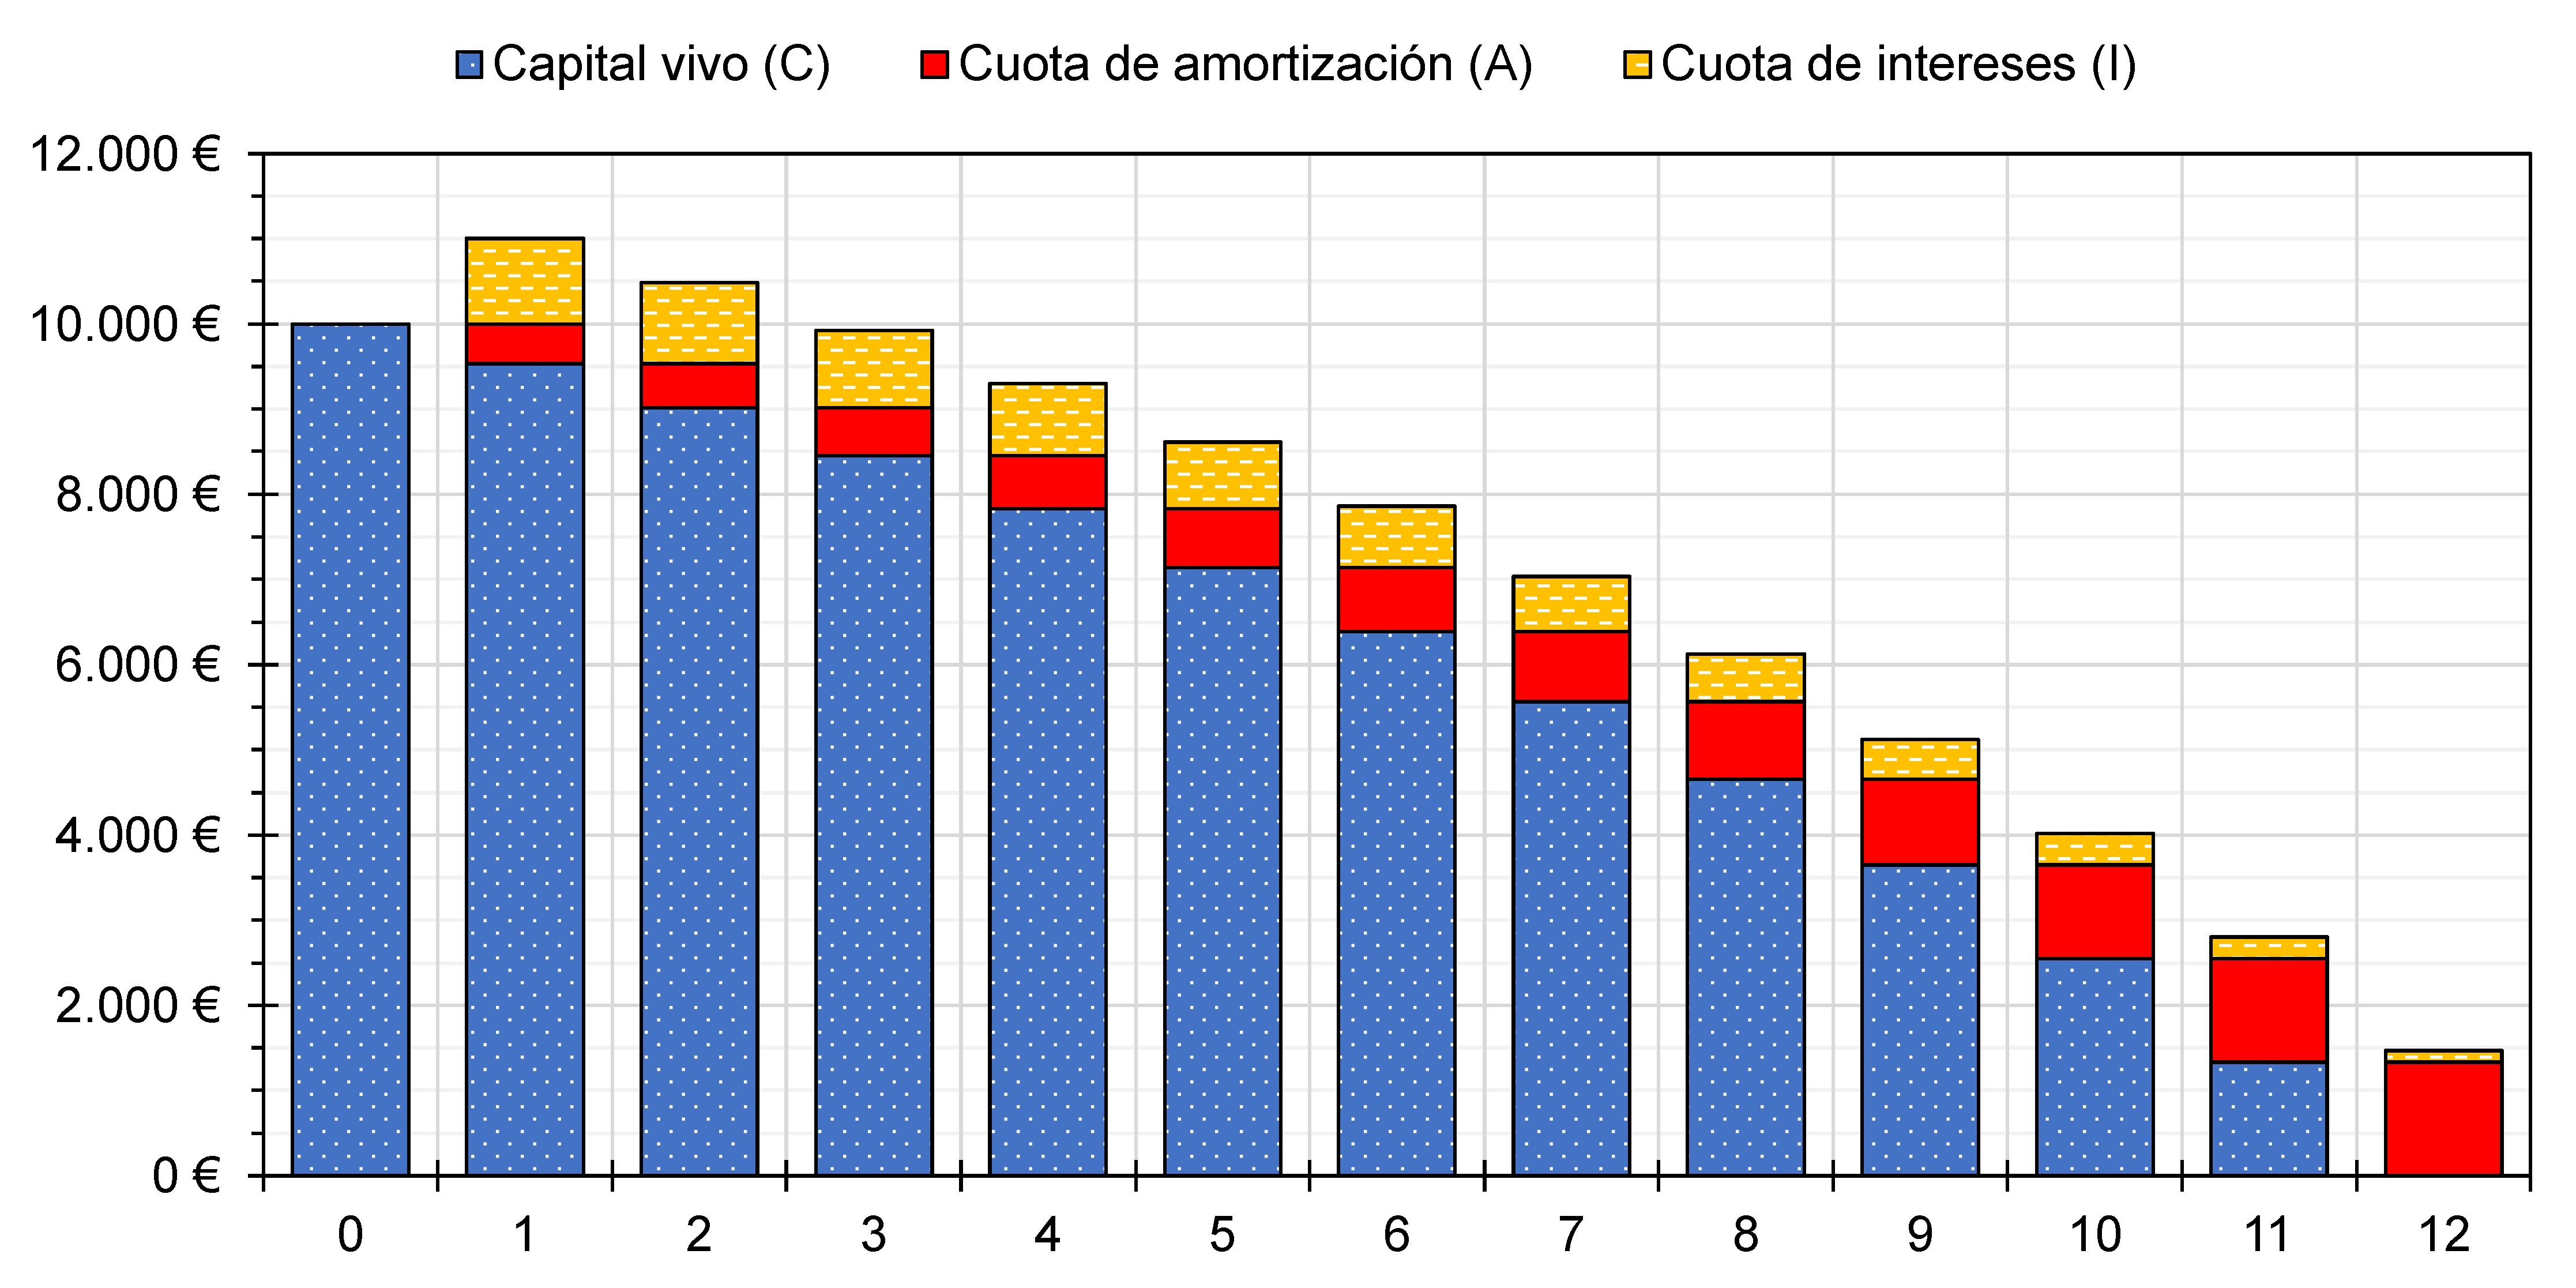
\includegraphics[width=11cm]{../figures/french-es.pdf}
\end{center}

\textbf{Préstamo americano}: el deudor sólo abona intereses al final de cada período excepto en el último, en el que abona además el nominal del préstamo, las cuotas son sólo intereses, el capital vivo no varía hasta el último período.

\begin{center}
	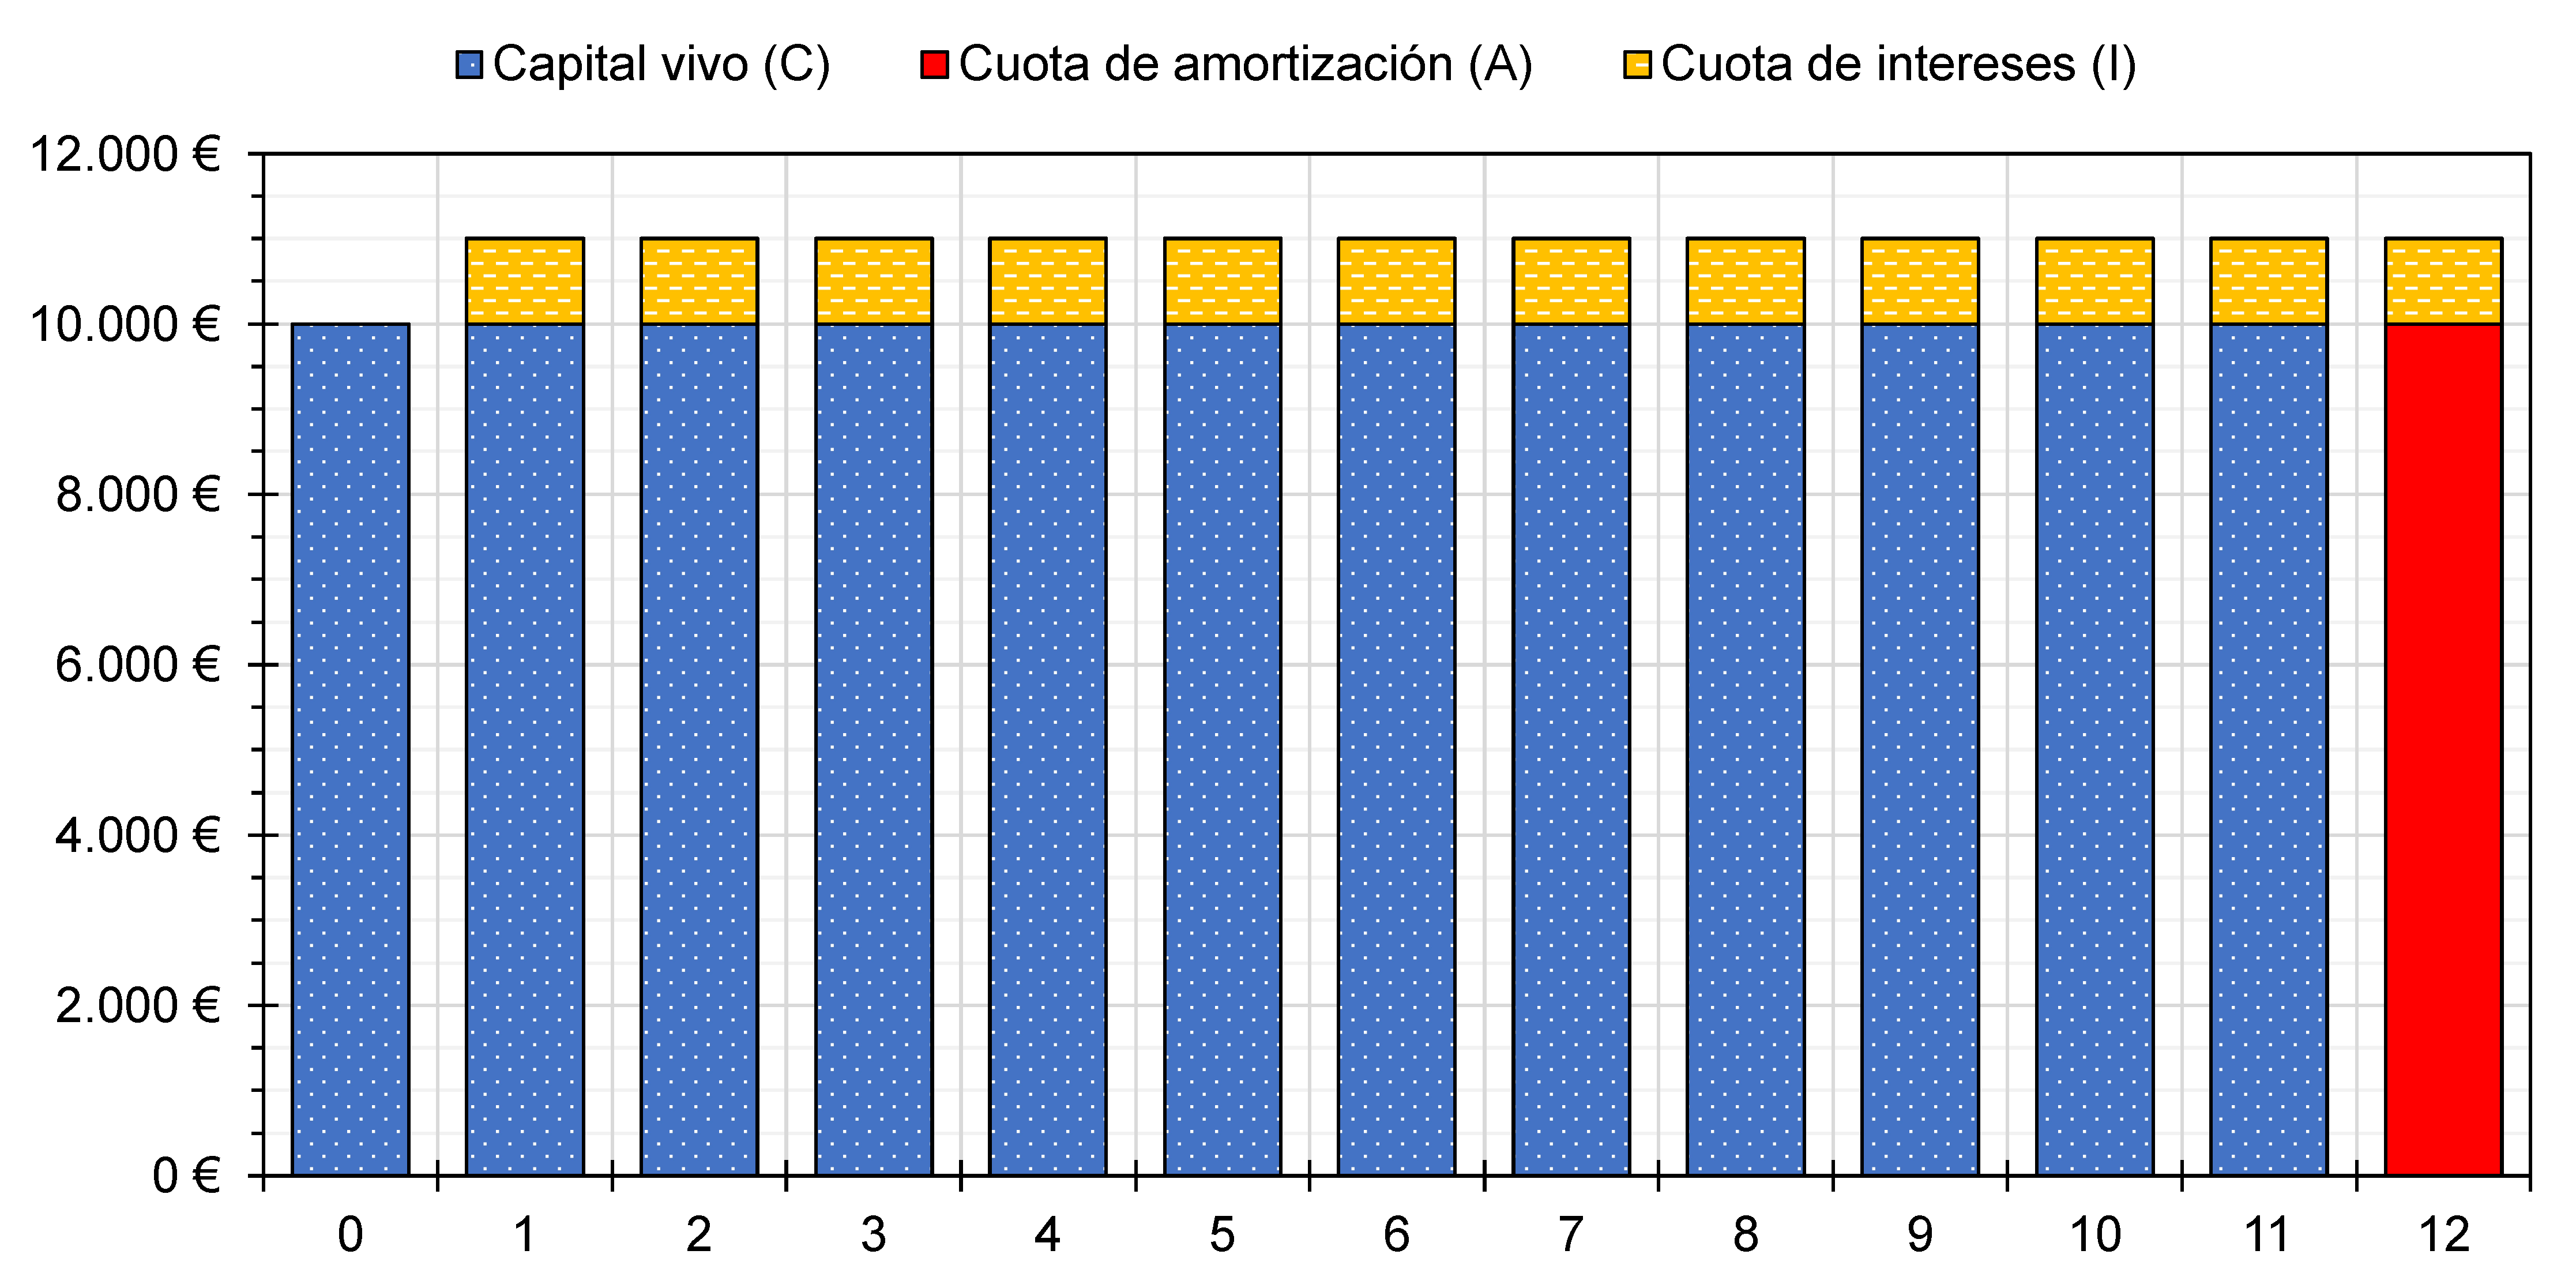
\includegraphics[width=11cm]{../figures/american-es.pdf}
\end{center}

\textbf{Préstamo italiano}: cuotas de amortización constantes, términos amortizativos y cuota de intereses disminuyen en progresión aritmética ($-i \cdot A$).	

\begin{center}
	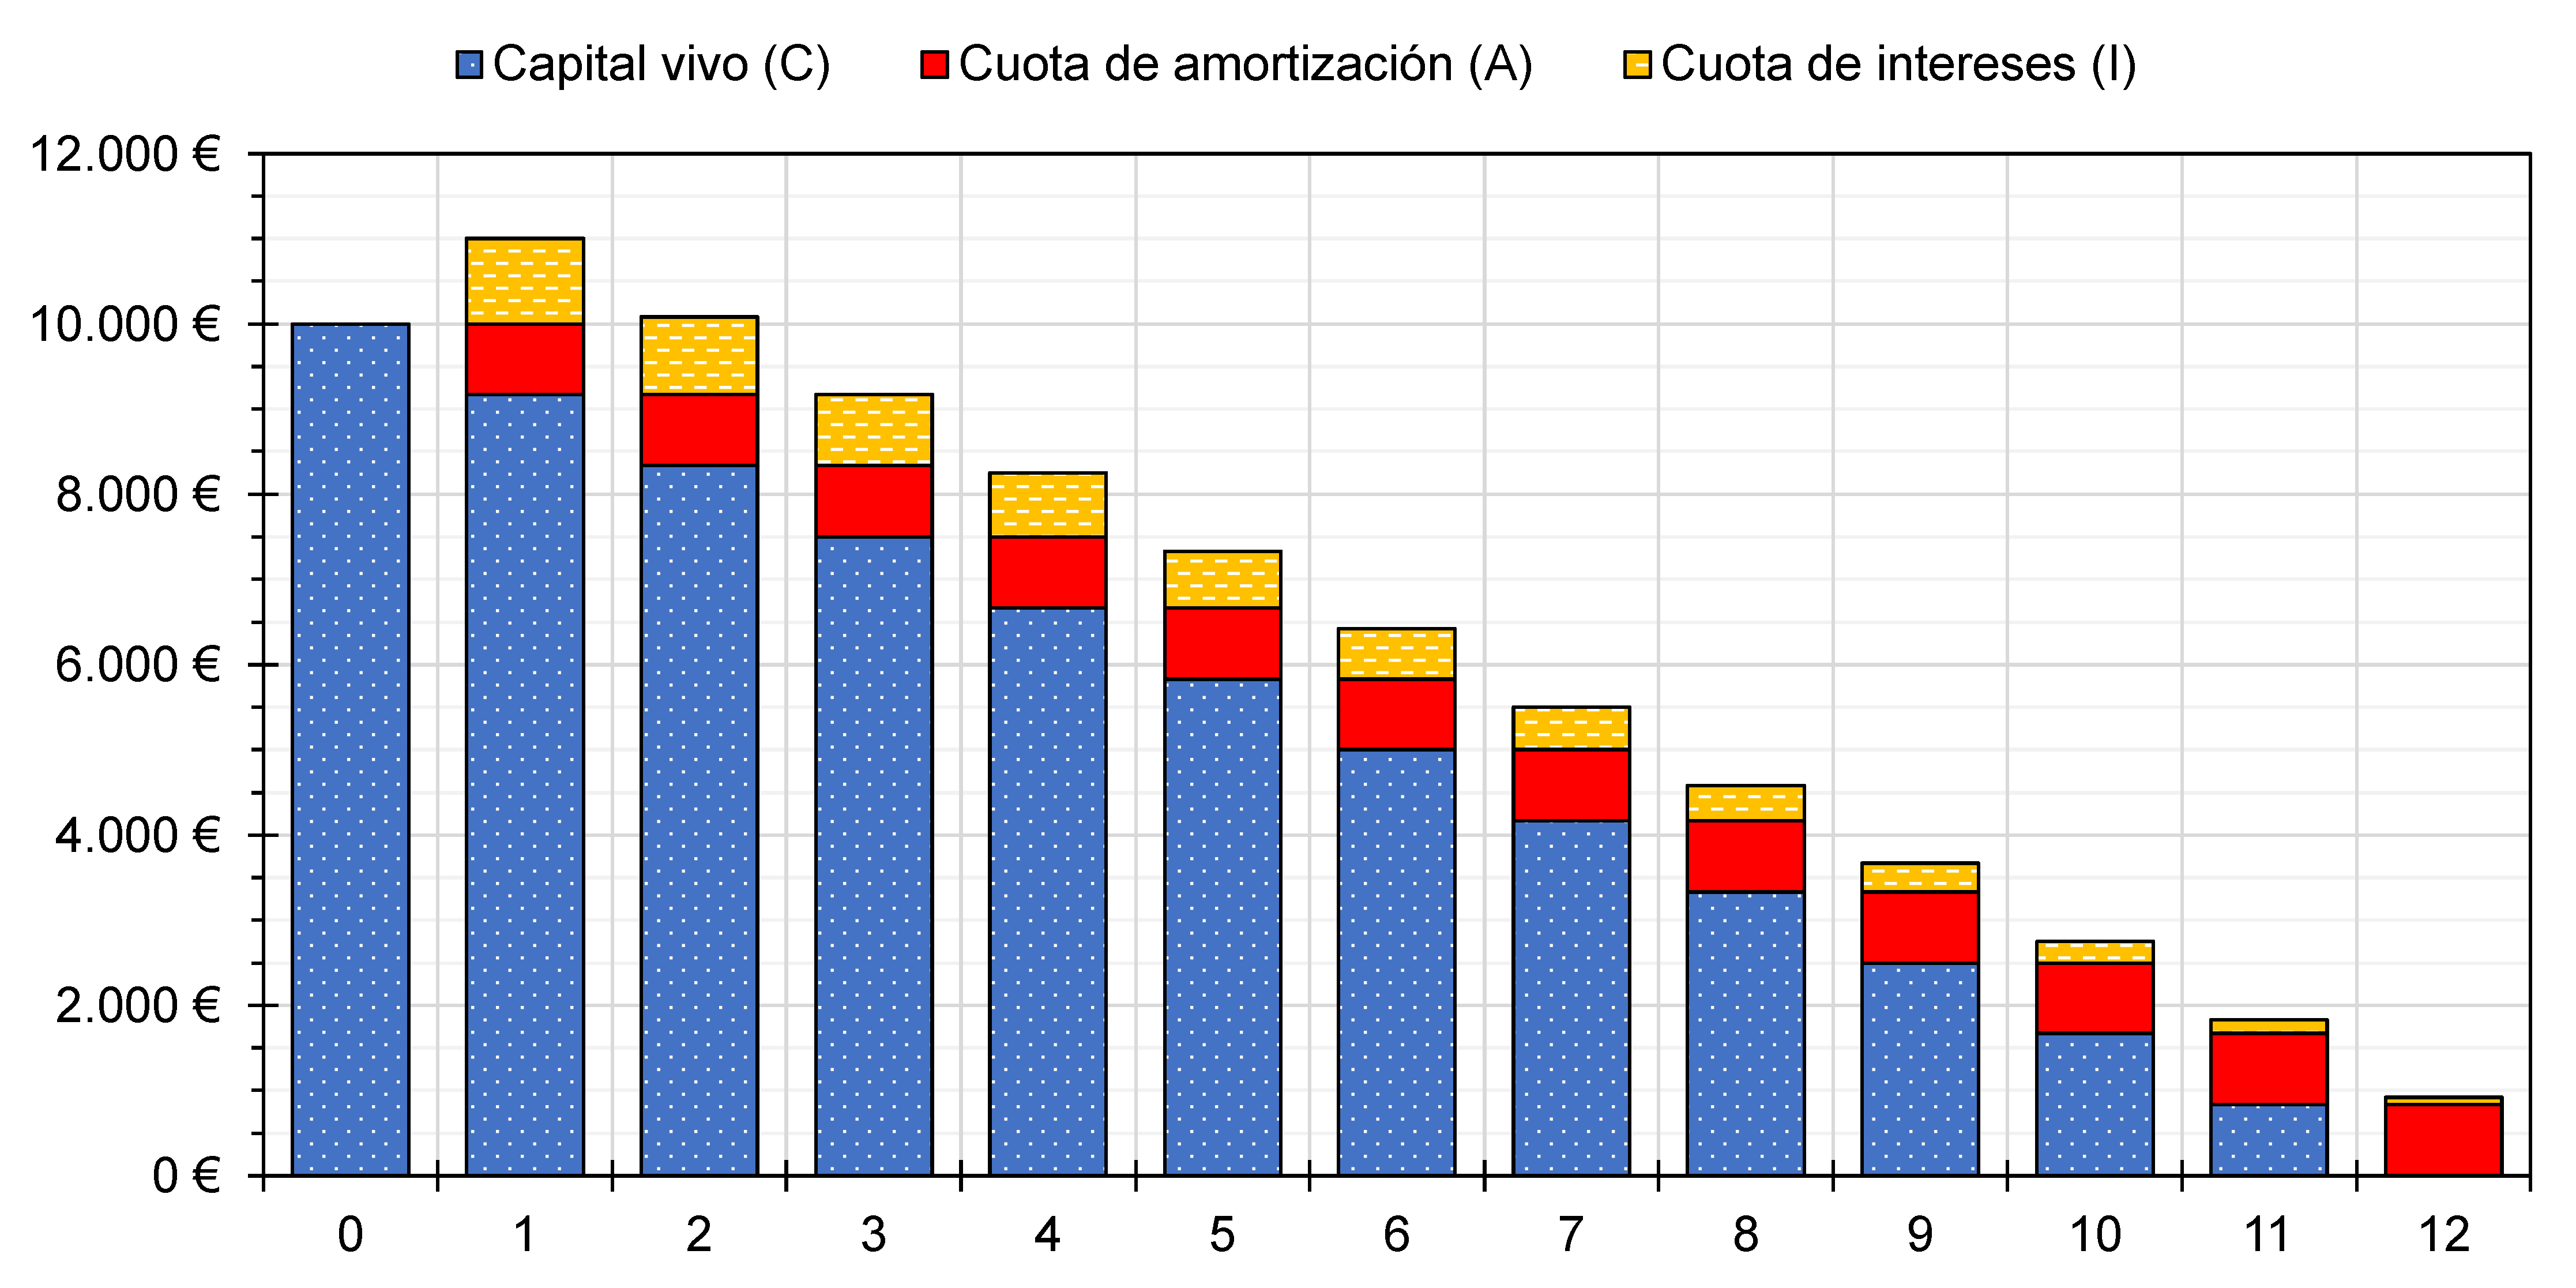
\includegraphics[width=11cm]{../figures/italian-es.pdf}
\end{center}

\textbf{Préstamo con términos en progresión geométrica}: términos amortizativos varían en progresión geométrica de razón $q$ (en este caso, $q = 1.05$).

\begin{center}
	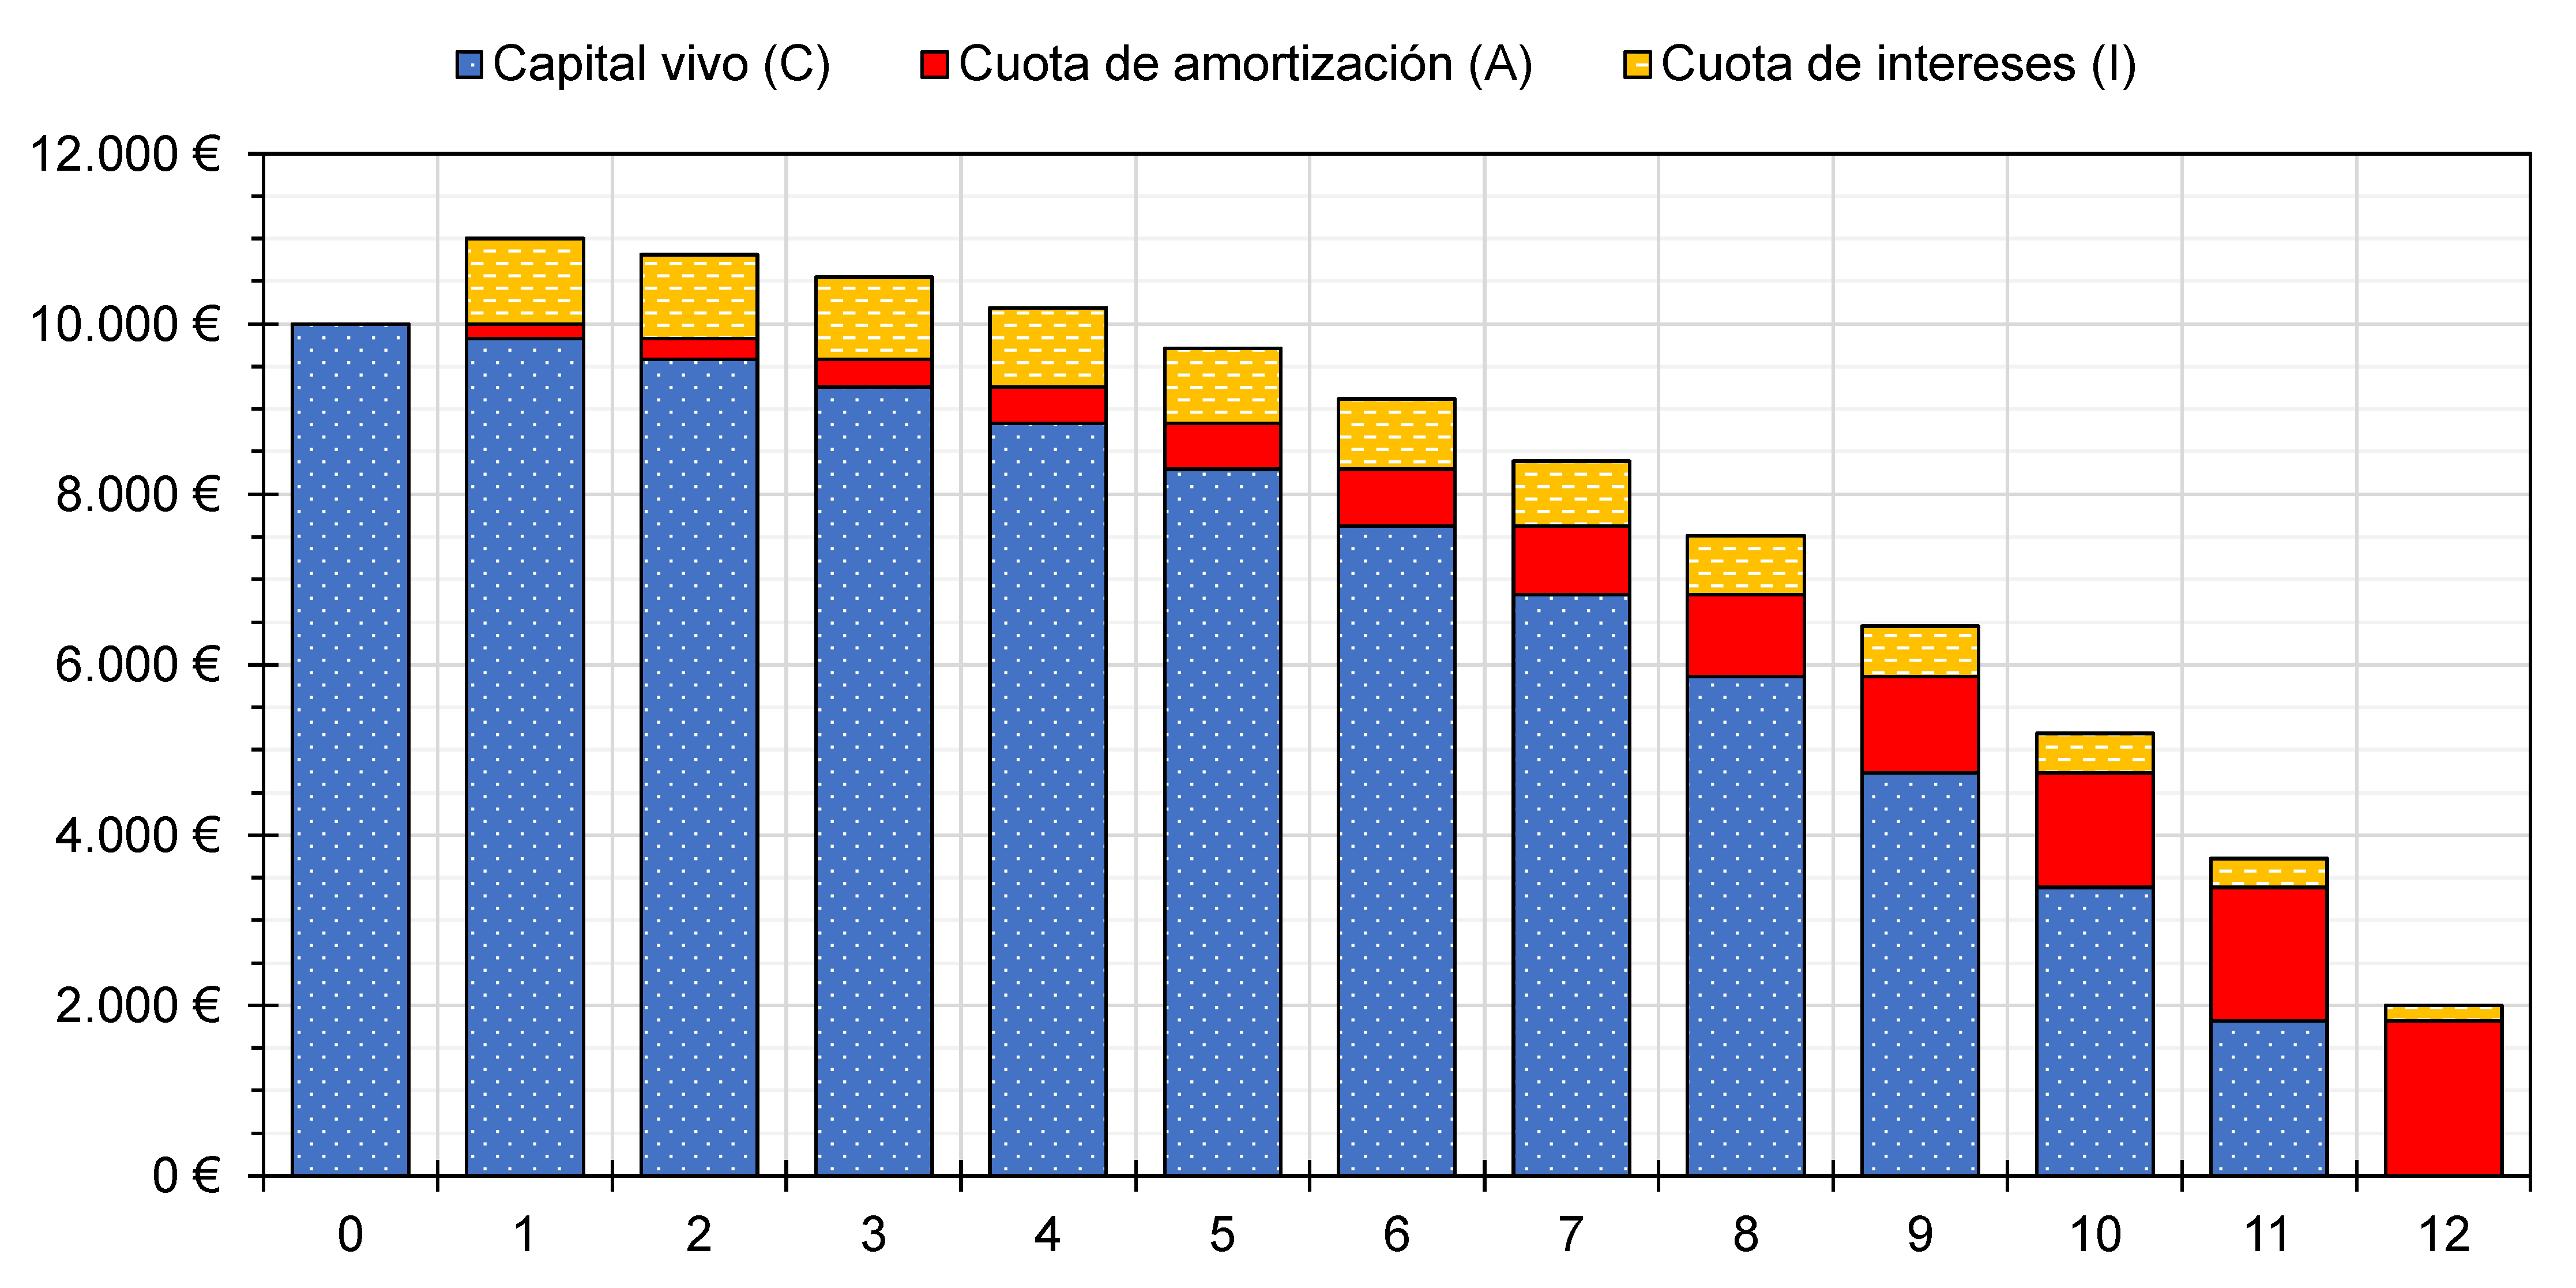
\includegraphics[width=11cm]{../figures/geometric-es.pdf}
\end{center}

\end{document}